\documentclass[journal]{IEEEtrancz}
% zvolte kodovani
\usepackage[utf8]{inputenc} % linux/unix
%\usepackage[latin2]{inputenc}
%\usepackage[cp1250]{inputenc} % Windows
\usepackage[czech]{babel}
\usepackage{graphicx}

\begin{document}

\title{Comparing various approaches to the mTSP problem}
\author{Teymur Azayev}

\maketitle

\begin{abstrakt}
We take a look at the mTSP problem and compare various approaches to finding approximate solutions, including local search, evolutionary algorithms, and an memetic search.
\end{abstrakt}


\IEEEpeerreviewmaketitle

\section{Task}
The Travelling Salesman Problem (TSP) is a task where given a number of cities we are looking for the shortest path that we can take while visiting all the cities only once and ending up at the city where we started at. 
This task can also be formalized as finding the shortest tour in a weighted non-oriented graph. \\
The mTSP task is a generalization to the TSP where we have multiple agents traversing the same graph. No agent is allowed to visit a city that has been visited by another agent.

\section{Introduction}
The mTSP, as the vanilla TSP problem are inherently NP-hard. We therefore have to use various approximate
optimization techniques which help us find an 'acceptable' solution to the problem.

\section{Goals}
The point of this report is to compare and benchmark local approaches with evolutionary algorithms in the mTSP
problem, and to discuss how various issues have been dealt with along the way.

\section{Implementation}
The problem is given by $n$ cities and $m$ agents. There is also an auxilliary city called the depot. Every agent
starts from and finishes at the depot. The solution is represented by two parts: A sequence of cities and a pair of boundaries for each agent. Each agent starts at the depot, then proceeds sequentially through the solution, beginning his boundary start index and finishing at his boundary stop index. From there the agent goes back to the depot. \\
The quality of the solution (and the fitness function) is taken as the longest route of all agents. This not only implicitly takes into account the total length of all tours of the agents, but normalizes the tour lengths so that they all approximately cover the same distance. We generate a concrete problem by randomly generating n points within a reasonable distance from the origin. We then run the algorithm and evaluate the solution after a certain amount of iterations. \\
As mentioned in the abstract, we use three different approaches to finding solutions for the mTSP.
The first approach is a simple local search algorithm. At every iteration we perform the following. We swap two of the cities in the sequence, evaluate the fitness and swap it back to how it was. This is done $n$ times
and the 'best swap' is recorded out of that iteration. The best swap is then performed and saved. \\
The second approach is a basic evolutionary algorithm on the same representation of the problem. 
A population of 200 is used at every iteration. The parents are selected using a standard roulette approach
and two new offspring are created using a one-point crossover operator. In order to produce a valid solution
every time we need to slightly modify the crossover operator. This is done by the offspring receiving part of the solution from one parent and sequentially recieving the rest of the sequence from the other parent such that the final sequence is valid. As a mutation, in each iteration we allow the boundaries of each agent to change with chance, meaning that each agent can have fewer or more cities in their path. The new offspring are accepted if they are better than their parents and accepted with a small chance if they are worse. \\
The last approach, the memetic algorithm simply extends the evolutionary algorithm by a local search at each iteration. This is done by using 2-opt on every new offspring after it is created. This is a method to let weak individuals locally improve and give them a chance to be selected in the next evaluation.




\section{Experiments}



\begin{figure}[ht]
  \centering
    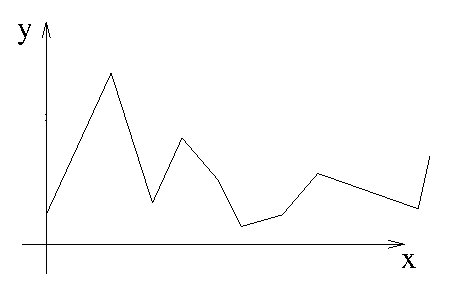
\includegraphics{figure}
      \caption{Název a stručný popis obrázku}
    \label{fig:exfig}
\end{figure}

Do experimetální části se přímo hodí obrázky. Každý obrázek musí být řádně vysvětlen
a okomentován. U grafů musí být popsány osy, pod obrázek umístíme název a 
krátké vysvětlení toho, co na obrázku je. Obrázek \ref{fig:exfig} je příklad
umístění obrázku do dokumentu.

\begin{table}
  \centering
  \caption{Parametry experimentu}
  \begin{tabular}{|l||c|c|c|}
  \hline
    & A & B & C \\
  \hline
  \hline
  S učitelem  & 0.22 & 0.27 & 0.29 \\
  \hline
  Bez učitele & 0.12 & 0.17 & 0.20 \\ 
  \hline
  \end{tabular}
  \label{tab:extab}
\end{table}

Výsledky experimentu je vhodné shrnout tabulkou, příkladem
je tabulka \ref{tab:extab}. Pro tabulku platí totéž co 
pro obrázek s výjimkou toho, že popis a název tabulky je nad tabulkou. Z tabulky
musí být jasné, co je jejím obsahem. Vysvětlení obsahu je vhodné uvést 
do textu poblíž tabulky.

\section{Diskuse}
Referát na tento předmět by neměl být větší než 3 strany v tomto formátu. 
Vlastní text by měl obsahovat úvod do problematiky zkoumaných dat, jejich rozbor. Návrh
použité neuronové sítě a v tabulce přehledné vstupní nastavení experimentu. Vždy je vhodné
uvést příklad zkoumaných dat, jaké obsahují atributy apod. Diskuse je důležitá kapitola,
která rozebírá dosažené výsledky. 

\section{Závěr}
Každý článek/referát musí obsahovat závěr, který stručně shrnuje dosažené výsledky 
experimentů. Závěr neobsahuje žádná nová zjištění, která by předtím v textu nebyla rozvedena.
Závěr je nejdůležitější část článku. Na základě závěru zpravidla pokrařujeme ve čtení
publikace. 


\begin{literatura}{1}

\bibitem{autor:rok}
Autor P., Autor M.: \emph{Název knihy}, druh literatury, 2002.

\end{literatura}
\end{document}
